\chapter{Methodology and Concept Development}
\label{chap:methodology}

This chapter presents the systematic approach taken in designing the Variant Management and Parametrization (VMAP) system. The methodology follows established software engineering principles to address the complex requirements of automotive parameter management. Beginning with a requirements analysis, the chapter proceeds to detail the conceptual architecture design, data model, validation mechanisms, and integration approaches developed to ensure system robustness and compatibility with existing enterprise infrastructure.

\section{Requirements Analysis}
\label{sec:requirements-analysis}

The foundation of the VMAP system design was a comprehensive requirements analysis combining stakeholder interviews, legacy system analysis, and industry best practice evaluation. This multi-faceted approach ensured the system would address actual user needs while overcoming limitations of existing approaches \cite{sommerville2011software}.

\subsection{Functional Requirements}
\label{subsec:functional-requirements}

The primary functional requirements derived from VMAP's fundamental purpose: replacing Excel-based parameter management with a centralized database solution. The system must support hierarchical organization of parameters within Electronic Control Units (ECUs), Modules, and Parameter IDs (PIDs), reflecting the domain-specific structure of automotive electronic systems \cite{staron2021automotive}. 

Users must be able to create variants for parameters with specific code rules determining their applicability, and define segments representing modified parameter values. If no segment exists, the system defaults to Parameter Definition Database values—an approach allowing efficient storage by tracking only modifications rather than duplicating unchanged parameters \cite{bhattacherjee2015principles}.

The system must track parameter values across four distinct release phases (Phase1, Phase2, Phase3, and Phase4), with changes in earlier phases propagating to later phases unless explicitly overridden. This phase-based approach represents a domain-specific adaptation particularly suited to automotive software development cycles \cite{broy2006challenges}.

All modifications require comprehensive logging with user information, timestamp, and detailed change data, supporting regulatory compliance and enabling parameter evolution tracking. The system must also provide functionality to create parameter configuration snapshots at specific points, particularly at phase transitions, for documentation purposes—an essential capability for quality assurance and regulatory compliance \cite{staron2021automotive}.

\subsection{User Role Requirements}
\label{subsec:user-role-requirements}

Analysis identified four distinct user roles with specific access requirements. Module developers require write access to parameters within their assigned modules, with the ability to create and modify variants and segments. Documentation specialists need access to frozen data for documentation, comparison capabilities between phases, and comprehensive change history access. System administrators require comprehensive control over user management, release phases, and special operations like variant deletion and phase freezing. Finally, read-only users need view access to all parameter data with parameter file generation capabilities but no modification rights.

These roles were defined based on the principle of least privilege \cite{sandhu1998role}, ensuring users have access only to functionality required for their specific responsibilities. This enhances system security while simplifying the user experience by presenting only relevant options. The hybrid role-permission model selected combines a primary role defining core permissions with additional permissions granted on a per-user basis, providing flexibility for special cases while maintaining a clear role structure.

\begin{figure}[h]
    \centering
    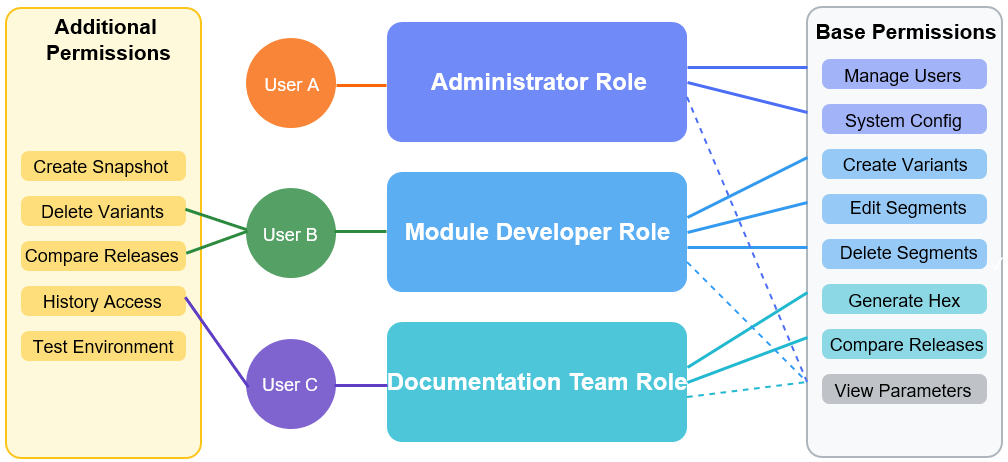
\includegraphics[width=0.95\textwidth]{figures/hybrid_role_permission_model.png}
    \caption{Hybrid Role-Permission Model}
    \label{fig:hybrid-role-model}
\end{figure}

Figure \ref{fig:hybrid-role-model} illustrates the hybrid role-permission approach that balances structured role assignments with flexible permission customization. This model supports both organizational clarity and individual access requirements.

\subsection{Data Management Requirements}
\label{subsec:data-management-requirements}

The system must maintain distinct parameter versions across different release phases, allowing simultaneous work on multiple phases while enabling access to parameter values from any development lifecycle point. Data integrity requires maintaining referential integrity across all related entities, particularly ensuring variants and segments associate with valid parameters \cite{elmasri2015fundamentals}.

Multi-dimensional parameter support is essential for complex automotive parameters such as mapping tables. Operations modifying multiple related entities must function as atomic transactions to maintain data consistency—particularly important for phase transitions where numerous parameters, variants, and segments may change simultaneously \cite{bhattacherjee2015principles}.

Query performance is critical, with efficient parameter data querying across dimensions including ECU, module, PID, release phase, and parameter name. These requirements influenced schema design decisions regarding normalization and indexing strategies to optimize common query patterns.

\subsection{Integration Requirements}
\label{subsec:integration-requirements}

VMAP must integrate with two external enterprise systems: the Parameter Definition Database (PDD) providing base ECU, module, PID, and parameter definitions; and the Vehicle Database supporting parameter file generation and variant code rule validation. The database must store necessary vehicle configuration data and maintain relationships between vehicle codes and variants, supporting practical application of parameter variants in vehicle-specific configurations \cite{staron2021automotive}.

These requirements follow enterprise integration patterns focusing on reliable data exchange, appropriate error handling, and minimal impact on existing systems \cite{hohpe2002enterprise}. The database implements these through specialized structures mapping between VMAP and external entities, tracking synchronization operations, and storing imported data with appropriate relationships to internally generated content.

\section{System Architecture Design}
\label{sec:system-architecture-design}

Based on the requirements analysis, a comprehensive system architecture was designed following a layered pattern with clear separation of concerns, enhancing maintainability while allowing independent component evolution \cite{fowler2003patterns}.

\subsection{Entity-Relationship Model}
\label{subsec:entity-relationship-model}

The entity-relationship (ER) model forms the foundation of the database design, capturing complex relationships between system entities. User management entities include Users, Roles, Permissions, and their relationships, implementing the hybrid role-permission model. Release management entities encompass Releases, Release Phases, and ECU Phase mappings, providing the foundation for version control. Parameter structure entities include ECUs, Modules, PIDs, Parameters, and Parameter Dimensions, representing the hierarchical organization of vehicle electronic systems \cite{staron2021automotive}.

\begin{figure}[htbp]
    \centering
    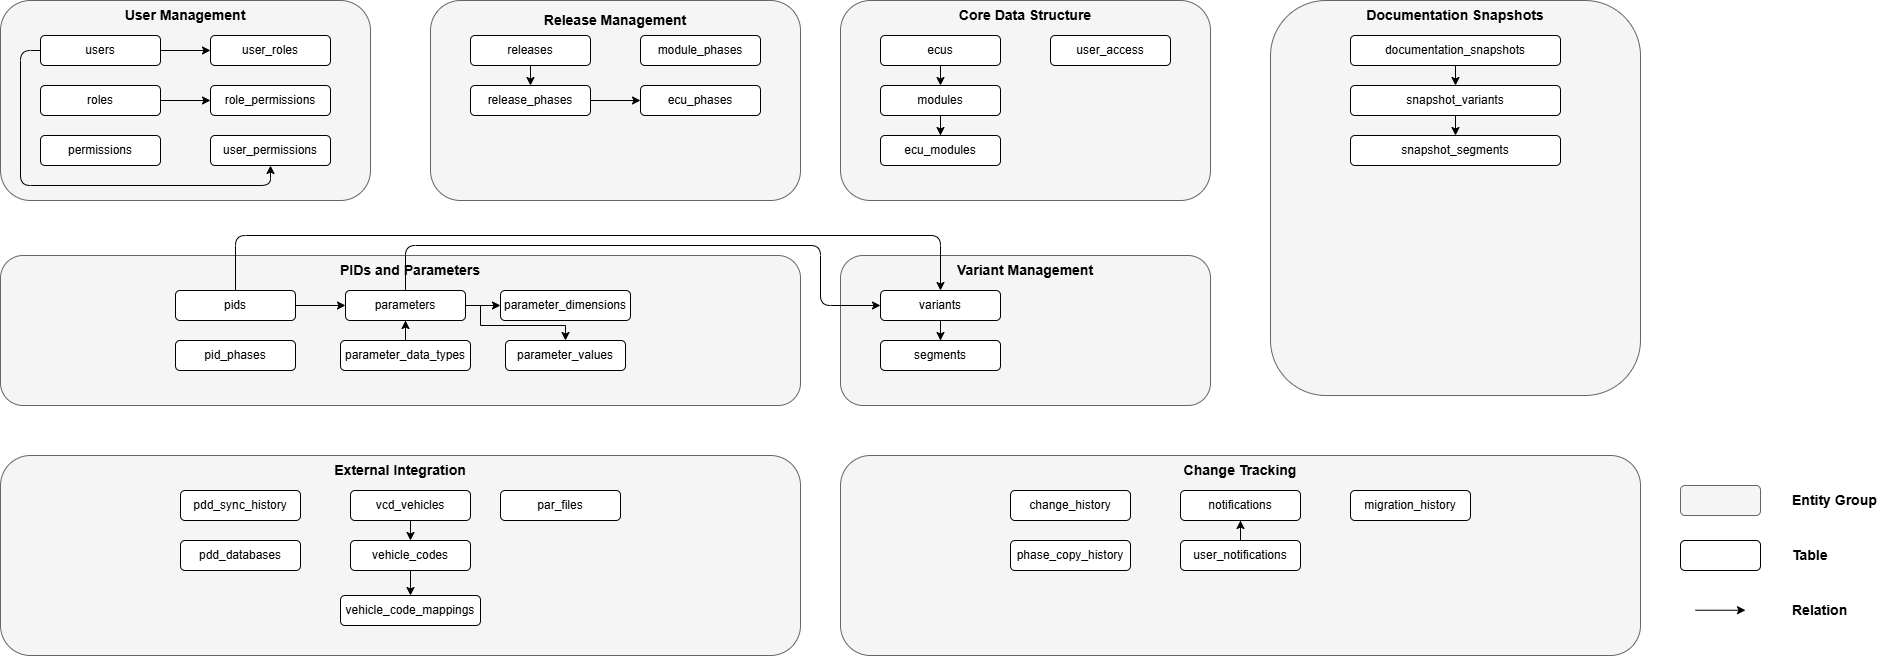
\includegraphics[width=0.95\textwidth]{figures/vmap_er_diagram.png}
    \caption{Entity-Relationship Diagram for VMAP Database}
    \label{fig:er-diagram}
\end{figure}

As shown in Figure \ref{fig:er-diagram}, variant management entities comprise Variants, Segments, and their relationships to parameters, implementing the core parameter customization functionality. Documentation entities include Documentation Snapshots, Snapshot Variants, and Snapshot Segments, supporting preservation of historical parameter states. Integration entities consist of Synchronization Records, Vehicle Configurations, and Parameter File Records, supporting external system connectivity. Finally, audit entities encompass Change History, Transaction Records, and Phase Copy History, providing comprehensive operation traceability.

This model was developed using data normalization principles to minimize redundancy while maintaining data integrity \cite{elmasri2015fundamentals}. Special attention was given to temporal data representation, incorporating bi-temporal database design concepts to track both transaction time and valid time \cite{kulkarni2012temporal}.

\subsection{Temporal Database Consideration}
\label{subsec:temporal-database-consideration}

Considerable attention was given to temporal database concepts as a potential foundation for the version control mechanism. The evaluation focused on bi-temporal modeling \cite{snodgrass1999developing}, which tracks both transaction time (when changes were made) and valid time (when changes are applicable).

% \begin{figure}[htbp]
%     \centering
%     %\includegraphics[width=0.9\textwidth]{figures/temporal_vs_phase_comparison.png}
%     \caption{Comparison of Temporal Database vs. Phase-based Versioning Approach}
%     \label{fig:temporal-comparison}
% \end{figure}

%As shown in Figure \ref{fig:temporal-comparison}, despite potential advantages including comprehensive historical preservation and flexible time-point querying, practical evaluation revealed significant limitations for automotive parameter management. Temporal queries' inherent complexity would introduce overhead potentially impacting interactive performance. The automotive development process organizes around discrete phases rather than continuous time, making the temporal model potentially misaligned with domain concepts. Temporal tables require additional columns and typically more rows to track historical states, substantially increasing storage requirements for a system with millions of parameter values. Effective temporal data querying requires additional indexes, further increasing storage overhead and potentially impacting write performance \cite{bohlen2018database}.
Despite potential advantages including comprehensive historical preservation and flexible time-point querying, practical evaluation revealed significant limitations for automotive parameter management. Temporal queries' inherent complexity would introduce overhead potentially impacting interactive performance. The automotive development process organizes around discrete phases rather than continuous time, making the temporal model potentially misaligned with domain concepts. Temporal tables require additional columns and typically more rows to track historical states, substantially increasing storage requirements for a system with millions of parameter values. Effective temporal data querying requires additional indexes, further increasing storage overhead and potentially impacting write performance \cite{bohlen2018database}.

Based on this evaluation, the system adopted an explicit phase-based approach rather than a temporal database model. This approach explicitly represents the phase-based structure of automotive development, making the model more intuitive for domain experts while supporting efficient parameter and variant retrieval without temporal query complexity \cite{bhattacherjee2015principles}. The phase-based approach better matches automotive parameter management's nature, where discrete development phases form the primary organizing principle rather than continuous time.

\subsection{Release/Phase Separation Rationale}
\label{subsec:release-phase-separation}

A key architectural decision was explicitly separating releases and phases into distinct but related entities. Releases represent major planning cycles in automotive development (typically aligned with model years or major updates like "24.1" or "24.3"), serving as organizational containers for development activities. Phases represent specific development process states (Phase1, Phase2, Phase3, and Phase4) occurring in a predictable sequence, reflecting parameter configuration maturity levels \cite{staron2021automotive}.

This separation provides several benefits: flexible release management allowing new releases with their own phase sequences without disrupting existing development; phase sequence standardization for consistent workflows; independent phase progression allowing different ECUs to advance through phases at different rates; simplified queries for common operations; and clear access control definition at either release or phase level.

The database schema implements this through distinct tables with a parent-child relationship. The releases table defines high-level development cycles, while release\_phases defines specific development states within each release with explicit sequencing. This structure enables efficient release-phase hierarchy navigation while maintaining clear semantic separation between these distinct concepts.

\subsection{Database Schema Design}
\label{subsec:database-schema-design}

The database schema translates the conceptual ER model into concrete database structures optimized for VMAP system requirements. PostgreSQL was selected as the underlying database management system due to its robust support for advanced features essential for this application domain, including complex data types (JSON/JSONB), sophisticated indexing mechanisms (including GIN indexes for text search), powerful procedural language (PL/pgSQL), comprehensive transaction support, and extensibility through custom extensions \cite{biriukov2018implementation}.

The schema addresses several key challenges in representing the automotive parameter domain. Parameters are organized hierarchically (ECU → Module → PID → Parameter) through related tables with appropriate foreign key constraints. Multi-dimensional parameters (arrays or matrices of values) are addressed through dedicated tables for parameter dimensions. Instead of traditional temporal database approaches, a phase-based versioning approach associates each parameter, variant, and segment with a specific phase and maintains phase sequence through explicit numbering.

Comprehensive change tracking is implemented through a specialized change history table capturing both old and new values for each change, using JSONB for flexible storage of different entity structures, grouping related changes by transaction, and supporting efficient filtering by entity type, user, and timestamp. This approach balances comprehensive auditing with performance considerations \cite{bhattacherjee2015principles}.

\subsection{Version Control Mechanism}
\label{subsec:version-control-mechanism}

The version control mechanism is central to VMAP, enabling parameter evolution management across different development phases. Unlike traditional version control systems focusing on linear history, VMAP implements a phase-based approach tailored to the automotive development process.

The release phase framework defines a structured parameter versioning approach based on the established automotive development cycle: Phase1 (initial definition and configuration), Phase2 (adjustments based on initial testing), Phase3 (refinement based on extended testing), and Phase4 (completed configuration ready for production).

This framework is implemented through table structures and procedural logic. Each phase is a distinct database entity associated with releases through a parent-child relationship. Parameters, variants, and segments are tagged with their corresponding phase, enabling explicit versioning without temporal database approach overhead. Explicit phase sequence numbers enable orderly progression, supporting both the development workflow and database operations propagating changes between phases.

The phase transition mechanism handles parameter configuration copying from one phase to the next through a specialized stored procedure. This approach provides several advantages: phases can be modified independently after copying; changes can be propagated forward selectively; each phase maintains a complete parameter configuration; and historical phase data remains accessible indefinitely.

A phase freezing mechanism supports documentation and regulatory compliance. When a phase is frozen, all parameters, variants, and segments become read-only, the frozen state is recorded with timestamp and user information, documentation snapshots are automatically generated, and the change is logged. This ensures significant development milestone configurations are preserved while allowing development to continue in subsequent phases.

\subsection{Parameter Definition Database Synchronization}
\label{subsec:parameter-db-sync}

Parameter Definition Database (CDI) synchronization presented complex architectural challenges. Initially, a version-based approach was considered, tracking parameter changes across releases by storing release information at synchronization. The system would dynamically construct appropriate parameter sets by evaluating parameter version histories. This approach offered theoretical storage efficiency advantages by maintaining only parameter changes rather than complete sets for each release \cite{bhattacherjee2015principles}.

\begin{figure}[htbp]
    \centering
    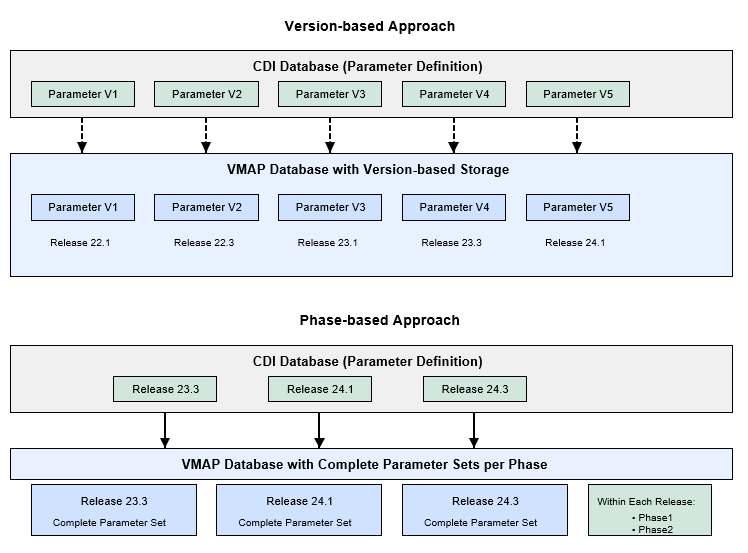
\includegraphics[width=0.9\textwidth]{figures/param-sync-approaches.png}
    \caption{Comparison of Version-based vs. Phase-based Parameter Synchronization Approaches}
    \label{fig:param-sync-approaches}
\end{figure}

Figure \ref{fig:param-sync-approaches} illustrates the comparison between the initially considered version-based approach and the implemented phase-based approach. Detailed analysis revealed significant challenges with versioning. Complex relationships between parameters and their parent entities would require sophisticated versioning logic for the entire hierarchy. Reconstructing parameter sets would require multiple joins across version tables and complex temporal predicates, potentially degrading system responsiveness. Additionally, version-based synchronization would complicate phase inheritance implementation \cite{kulkarni2012temporal}.

After evaluation, a phase-based synchronization approach was adopted instead. This design maintains complete parameter sets for each ECU in each release phase, rather than tracking individual parameter versions across releases. This simplifies query patterns by establishing direct relationships between parameters and their release phases, enables efficient retrieval without complex version reconstruction, aligns naturally with the automotive development process, provides clearer traceability between parameter versions across phases, and offers greater resilience against synchronization failures \cite{hohpe2002enterprise}.

While this approach consumes more storage than a version-based approach, detailed analysis indicated storage requirements remained within acceptable limits, with performance benefits and simplified implementation outweighing additional storage costs.

\section{Validation Mechanisms}
\label{sec:validation-mechanisms}

To ensure data integrity and consistency, VMAP implements multiple validation mechanism layers from basic constraints to sophisticated business rule validation. These layers work together to maintain parameter data quality and reliability throughout the system lifecycle.

\subsection{Data Integrity Constraints}
\label{subsec:data-integrity-constraints}

Database-level constraints enforce basic integrity rules: primary key constraints ensure unique entity identifiers; foreign key constraints maintain referential integrity between related entities; not-null constraints ensure required fields contain values; unique constraints prevent duplicate values in specified columns; and check constraints enforce domain-specific rules such as valid date ranges and parameter value ranges. These constraints are designed into the database schema as integral parts of entity definitions, ensuring consistent enforcement throughout the system \cite{elmasri2015fundamentals}.

\subsection{Business Rule Validation}
\label{subsec:business-rule-validation}

Domain-specific business rules are implemented through database triggers and stored procedures. Parameter range validation automatically checks modified values against defined minimum and maximum bounds, rejecting values outside allowed ranges—critical for automotive parameter management where incorrect values could impact vehicle safety or performance \cite{staron2021automotive}.

Phase status validation prevents frozen phase modification, ensuring historical parameter configuration integrity. Segment validation ensures segments reference valid parameters and variants, contain appropriate dimensional values, and maintain consistent entity relationships. User access validation ensures users can only modify parameters, variants, and segments for modules to which they have been granted access, maintaining data security and integrity in multi-user enterprise systems \cite{sandhu1998role}.

\subsection{Conflict Resolution Strategies}
\label{subsec:conflict-resolution-strategies}

In a multi-user environment, concurrent modifications can create conflicts. VMAP implements several strategies to detect and resolve these, maintaining data consistency while supporting collaborative parameter management. For web-based interactions, optimistic concurrency control using version timestamps allows multiple users to view the same data concurrently, detecting conflicts only when updates collide \cite{bhattacherjee2015principles}.

When changes propagate from one phase to the next, conflicts can arise if the target phase has already been modified. Explicit conflict resolution mechanisms compare the source variant or segment with existing target configurations during phase propagation operations. When conflicts are detected, resolution options allow users to make informed decisions: override the target with source values, preserve target values, or merge values based on specified rules.

Complex operations modifying multiple related entities use explicit transactions to maintain data consistency. Database transactions ensure related modification sets either complete entirely or fail without partial changes. For operations spanning multiple transactions or requiring user interaction, application-level coordination through transaction identifiers and session state enables complex workflows requiring user input while maintaining logical data consistency.

\subsection{Audit and Traceability Mechanisms}
\label{subsec:audit-mechanisms}

Comprehensive audit and traceability mechanisms are essential for regulatory compliance and quality assurance. VMAP includes robust audit capabilities tracking all significant operations while minimizing performance impact. The core is the change history tracking mechanism, automatically capturing both before and after states for entity modifications. For each change, the system records the entity being modified, change type, user, timestamp, and detailed before/after values \cite{bhattacherjee2015principles}.

\begin{figure}[h]
    \centering
    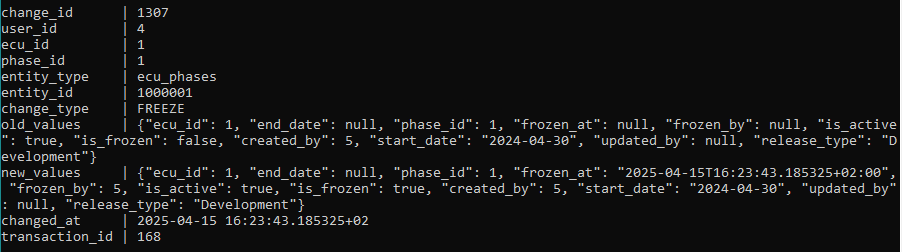
\includegraphics[width=0.95\textwidth]{figures/freeze_audit_trail.png}
    \caption{Audit Trail for Phase Freeze Operation}
    \label{fig:freeze-audit-trail}
\end{figure}

Figure \ref{fig:freeze-audit-trail} shows an example of the audit trail for a phase freeze operation, demonstrating the comprehensive tracking of significant system events. To optimize performance, the audit system selectively filters change data, excluding non-essential fields such as timestamps and large binary data. Additionally, asynchronous audit recording for bulk operations reduces performance impact on high-volume operations while ensuring all changes are eventually recorded.

Beyond change tracking, specialized audit mechanisms address specific scenarios: phase transition logging records all phase propagation operations; freeze operation logging records phase freeze and unfreeze operations; user access logging captures authentication and authorization events; and integration operation logging records all external system interactions.
